


\subsection{Overview of the \lasi~system}

The \lasi~system \cite{ref:lasercalvet} was composed of three main parts: optical, calibration and electronics.

\begin{figure}[htbp]
\centering
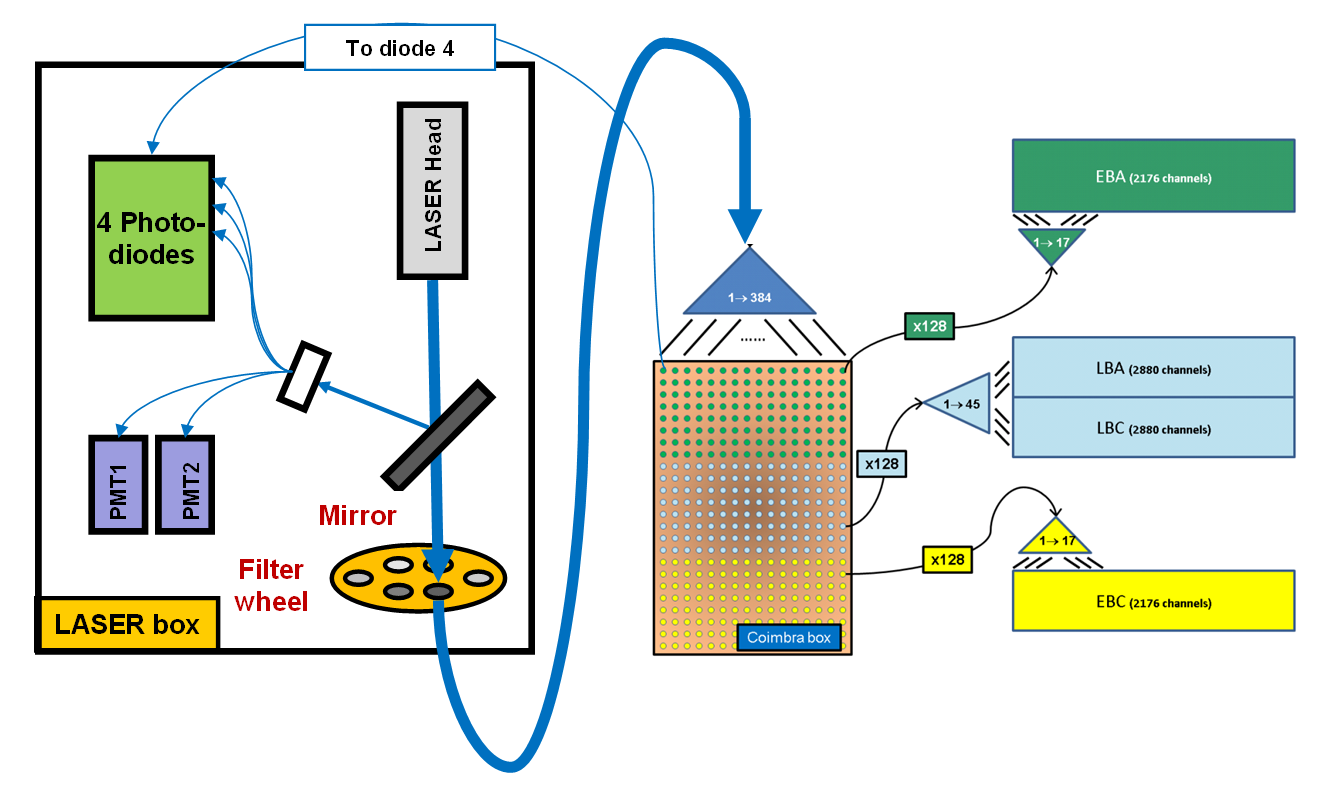
\includegraphics[height=7cm]{figures/FullSystem.png}
\caption{Sketch of the optical part of the \lasi~system. At first 3 photodiodes were measuring the light before the filter wheel and one photodiode was plugged after the \coimbra~box. The final configuration was different: one photodiode before the filter wheel and three after the \coimbra~system.}\label{fig:lasaoptical}
\end{figure}


\begin{itemize}
\item optical part 

	The optical part of the \lasi~system is sketched on Figure \ref{fig:lasaoptical}. It was composed of three parts:
	\begin{itemize}
	\item the \las~box (Fig. \ref{fig:lasabox}): the light emitted by the diode pumped solid state \las~from SpectraPhysics (green beam with $\lambda$ = 532 nm) was splitted by a semi-reflecting mirror. A small amount of the light (about 9\%) was sent to a light-mixing block, composed of reflective filters, light diffusers and a light mixer, and transmitted to a bundle of 9 fibers. \par
		\begin{figure}[htbp]
			\centering
			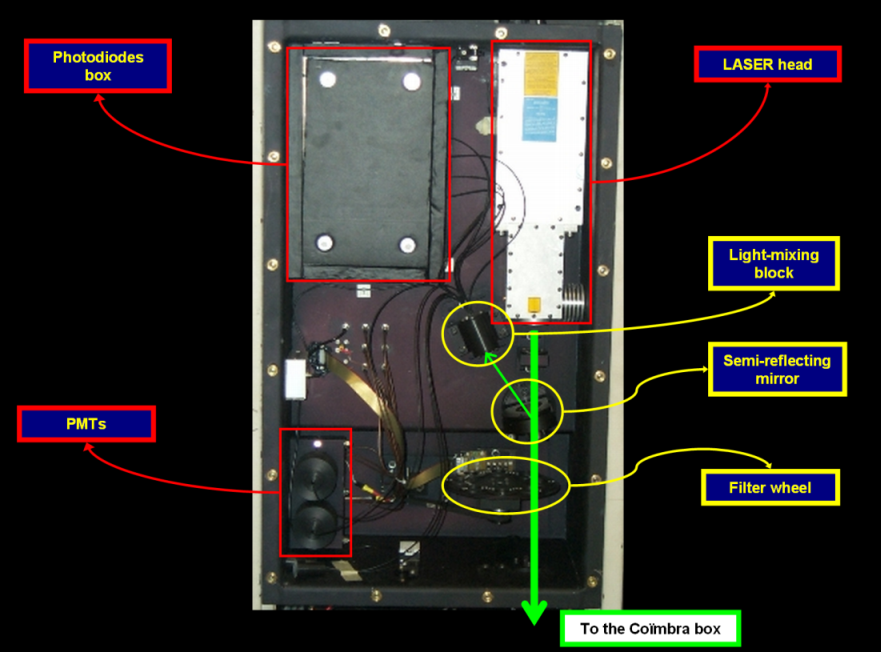
\includegraphics[height=7cm]{figures/LaserBox.png}
			\caption{Picture of the \las~box of the \lasi~system}\label{fig:lasabox}
		\end{figure}	
			
		Two of these fibers were connected to two \pmts, used for timing purposes (trigger), and one was linked to a photodiode to ensure an absolute measurement of the light. The other part of the \las~light was sent to one of the attenuating filter located on a wheel and then to a liquid fiber that transmitted the output light to the \coimbra~system. \par
                 The \las~box was equipped with a custom-built electromechanical shutter for safety purpose. This semi-passive component aimed at isolating the \las~box from the \tilecal: the \las~light was transmitted only to the optical components of the box and not to the \pmt~of the \tilecal. 

	\item the \coimbra~box : this system was transmitting the light coming from a liquid fiber to a bundle of long clear fibers that were connected to the \pmts~of the \tilecal. It was composed of a divergent lens, an unpolished acrylic disk (used as a diffuser), and a convergent lens.
	\item clear fibers of about 100 to 120 m long transfer the light coming out of the \coimbra~box to the 9852 \pmts~of the \tilecal. There were 400 fibers (1 fiber for two half-modules for the central calorimeter, 1 fiber for each half-module of the extended barrels, and 16 spare fibers). 
	\end{itemize}
		
\item calibration part 
	
	The photodiode box, located inside the \las~box, housed four photodiodes and their electronics calibrated with an Americium $\alpha$-source (3.7 kBq). The box temperature was regulated with Peltier modules and the humidity was controlled via an air dry flow. The inter-calibration of the photodiodes was performed regularly via specific runs with the embedded source moving along the photodiodes. 
	
\item electronics part 
	
	The set of electronics modules used to control and command the \lasa~system is shown on figure \ref{fig:lasaelectronics}. It was housed inside a VME crate and was composed of the following modules:
	\begin{figure}[htbp]
			\centering
			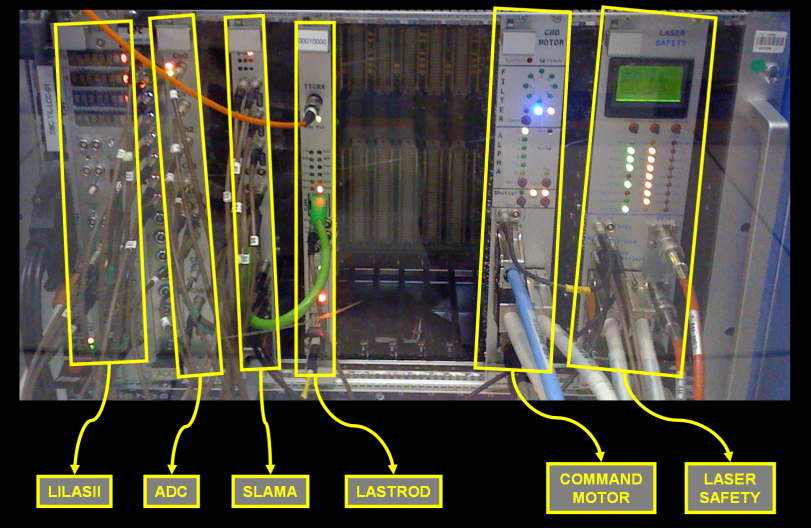
\includegraphics[height=7cm]{figures/Electronics.png}
			\caption{Picture of the electronics part of the \lasi~system}\label{fig:lasaelectronics}
		\end{figure}	
		
	\begin{itemize}
	\item {\sc LILASII}: dedicated to the measurement of the linearity of the electronics of the photodiodes,
	\item {\sc ADC}: to convert the \las~box analog signals (from the two \pmts~and the four photodiodes) into digital ones,
	\item {\sc SLAMA}: system command (trigger) and communication with \atlas,
	\item {\sc LASTROD}: \las~\tilecal~ReadOut driven: to send the \las~data to \atlas DAQ,
	\item {\sc MOTOR COMMAND}: used for mechanical commands (wheel of filters, shutter, radioactive $\alpha$-source),
	\item \las~safety: system monitoring and control (DCS, interlocks).
	\end{itemize}
	
\end{itemize}



\subsection{Performance}
A monitoring of the various components of the \lasi~system was performed regularly and its performance evaluated.  The measurements considered were:
\begin{itemize}
\item{pedestal runs} 
	
	Pedestal may be estimated with dedicated runs or during the calibration runs (with the $\alpha$-source). Significant variations may show potential electronics problems. A stability better than 0.5\% has been observed on the mean pedestal values \cite{ref:laserb}.
\item{photodiode stability monitoring}
	
	The monitoring was performed during the calibration runs with the $\alpha$ source. The mean of the photodiodes signal has been chosen to monitor the stability, which was about 0.15\% over few months.
	
\item{linearity of the electronics of the photodiodes}
	
	The linearity of the electronics of the photodiodes was performed through {\sc LILASII}. A known charge was injected to the electronics (preamplifiers, ADC and the related electronics chain) that digitized the photodiode signals. An additional ADC channel was used to digitize the charge injected. 
\item{PMT/Diode ratio in the \las~box}
	
	The two \pmts~of the \las~box were primarily used for triggering purpose. But they may also be part of the stability surveys of the \las~system through the study of the ratio of the \pmts~signal to the Diode1 one. Over a few months period, a stability at the level of 0.6\% has been observed \cite{ref:laserb}.
	
\item{\tilecal~channels stability monitoring}
	
	This was the main purpose of the \las~system: monitoring the behavior of the 9852 \pmts~of the \tilecal~and pointing at possible drifts. Signals from the \pmts~may be normalized to diode measurements so as to minimize the instabilities of the intensity of the light emitted by the \las.  \par
	For each \pmt~the ratio $f_{las}={{PMT~signal}\over{Diode1~signal}}$ was estimated for a \las~reference run, defined as the first \las~run performed after a Cesium scan, and for a given run. A fiber-to-fiber correction was applied to compensate for light instabilities and inhomogeneities, which accounted for the main source of systematic uncertainties. The channel variation may be estimated from ${{f_{las}^{run}}\over{f_{las}^{ref}}}-1$ and a stability at the level of 0.6\% has been observed over a few month period.
	
	
\end{itemize}


\subsection{Shortcomings}
The \las~system installed in USA15 has shown very good performance. Nonetheless few shortcomings have been observed and may be solved to get an even better system:
\begin{itemize}
\item{\coimbra~box instabilities} 
	
The amount of light sent to each of the 400 fibers coming out of the \coimbra~system must be very stable in time, since this signal that was used to estimate the stability of the \pmts~of the \tilecal. But a decrease of the light in the fibers of about 4\% over a period of 1.5 month has been observed. This effect was is handled via software corrections but understanding and solving this problem would allow a gain of sensitivity of the system.
	
\item{Photodiode box grounding problem} 
	
During an $\alpha$-source run, it has been shown that, when the source is in front of a given photodiode, the pedestals measured by the other photodiodes are not the same as the ones measured during a pedestal run, when the source is located in its garage position. This problem was related to cross-talk of the ground. It has been solved by re-designing the bus card along which transit the low voltages for the electronics of the photodiodes and the signals coming from the preamplifiers. This new card has been installed in USA15 in 2011. \par
Another effect has been observed: when photodiodes are illuminated all at a time by a \las~signal with a given intensity, the signal seen by the electronics for a given photodiode differs significantly from the one measured when only this photodiode receives a \las~light of the same intensity. This optical cross-talk had already been observed in 2009, and was attenuated in the following way: when a given photodiode is illuminated with a \las~light corresponding to a given intensity, all other photodiodes are operated in reverse polarization.
		
\item{Filters non-uniformity}
	
The filters used to increase the \las~dynamic range were inserted into a moving wheel. The reproducibility of the position of the wheel has been estimated by performing consecutive \las~runs at a given intensity after a rotation of the wheel. An effect at the level of few \% has been observed. This could be measured and corrected with photodiodes inserted between the rotating wheel and the \coimbra~box.
	
\item{Electronics}

Some problems that may be related to \lasi~electronics have been observed. From time to time LASTROD was found desynchronized with the LHC clock. Even if the origin of the problem has never been clearly identified, it seems clear that the number of electronic boards does not tend to ease the synchronization and signal transmissions. The \lasi~electronics was containing 11 Field Programmable Arrays (FPGA) (with the following distribution : LASTROD : 4, SLAMA : 3, LILAS : 1, QDC : 1, Motor : 1, Safety : 1) and this did not ease the management of the many signals spread over the system. Furthemore FPGAs were not as efficient (in terms of frequency or memory) when the \lasi~system was built as they are nowadays. In particular the memory of SLAMA's FPGA was filled at the level of more than 80\% making difficult to manage an increase of information that may be due to hardware upgrades.  



\end{itemize}
